\chapter{Developing Unplagged}\label{chap:developingUnplagged}

Coming from the \nameref{chap:systemRequirements} here we have yet another set of requirements, before we can
start with the actual description of the way you can help us develop the system. This time it's 
about what we believe will be helpful or sometimes even necessary prerequisites. 

First of all, the programming languages mostly used in Unplagged are PHP and JavaScript, both of which in conjuction
with a framework. Teaching programming languages is, as you probably can imagine, well beyond the scope of this document,
but we will at least try to cover the most important concepts of the frameworks as they occur. 

The used frameworks are 
\href{http://jquery.com/}{jQuery} for Javascript and \href{http://framework.zend.com/docs/overview}{ZEND} for PHP 
respectively. jQuery is kind of the industry standard for unobtrusive scripting with about 50\% 
of the Top 10.000 websites using it according to \citet{Trends} and the Zend framework is also well established and
brings a lot of features, that are useful to this project.

For most of the other topics, we will give you some (hopefully) helpful resources on the way, if it isn't covered 
thoroughly by us. But just to let you
know, here is a list of the buzzwords, er technologies that will be mentioned:

\begin{itemize}
\item Scrum
\item HTML5 and CSS3
\item Continuous Integration
\item Responsive Webdesign
\item Progressive Enhancement
\item Git, Netbeans, Redmine
\item Tesseract, Imagemagick
\item Simtext
\end{itemize}

As said in section \nameref{platforms}, the system is developed, so that it should work on multiple platforms. 
This makes it sometimes difficult to describe certain installation processes in a way that would work for everybody. As
it's often most problematic, to get some Linux software running on Windows, we will mostly concentrate on the way those
things are done on this platform and give the instructions for other operating systems as an aside if necessary.

\section{Development Environment}

The following parts will mostly focus on the way you can get a development version of unplagged up and running on your 
system.

\subsection{Git}
The source code and files of all parts of the Unplagged project are managed through Git, 
with the repository hosted at \href{https://github.com}{Github}. 
Git is a distributed version control system, that exists since 2005 and gained more and more 
track in recent years, because many developers prefer it over other version control system because of its simplicity. This
made it also interesting for us to use it for Unplagged. % citation?

However, none of the team memebers had ever used 
Git before in a bigger context so it was a challenge to get it running on all the systems. But we took it, to explore all the 
features Git offers. It is much easier to create different branches and merge them again, than it is with other 
version control systems like Subversion.

If you didn't use git before, it would probably be a good idea, to watch this 8 minutes Git introduction as a starting point:
% This feels weird, because it is actually described from the start afterwards, so why the video?

\begin{itemize}
\item \url{http://www.youtube.com/watch?v=RDGzF2M-zlo}
\end{itemize}

\subsubsection{Installating the Git Bash}

First of all let's find out, how to install the Git console application, called Git Bash. 
Unfortunately all the GUIs we were evaluating didn't work consistently, so we decided to use it from the command line 
only. 
A very good instruction on how to install the Git Bash can be found on the website of the github project:

\begin{description}
\item[Mac OS X:] \url{http://help.github.com/mac-set-up-git/}
\item[Windows:] \url{http://help.github.com/win-set-up-git/}
\item[Linux:] \url{http://help.github.com/linux-set-up-git/}
\end{description}

\subsubsection{Getting the source code of the unplagged project}
Now it is time to get the project source code on your machine. As said before, the whole unplagged project is hosted on 
github, so if you want to be able to contribute source code later on, you first need to create an account on \url{https://github.com}.
This isn't necessary, if you simply want to look into the source code, which can be accessed via \url{https://github.com/benoertel/unplagged}.

If you haven't been granted write access to the above mentioned repository by a project member (which is very likely when
you are reading this document for the first time), you will need to do a fork
of the Unplagged project right at github, like described in:

\begin{itemize}
\item \url{http://help.github.com/fork-a-repo/}
\end{itemize}

After this the following steps are mostly the same for everybody, with the distinction of the project URIs, which should 
be the one of 
your newly created fork.

Open up the Git Bash and switch to the directory where you want the project to be 
located and clone the repository:

\begin{lstlisting}[caption=Cloning a repository]
cd ?Sites/unplagged.local?
git clone ?https://<username>@github.com/benoertel/unplagged.git?
\end{lstlisting}

After this you should have a local copy of all the repository data in the specified directory.

\subsubsection{The most important git commands}

You are now ready to use Git! Here are some more instructions on the most important commands and how to properly use it. 
However, if the given instructions in this manual are not enough, feel free to checkout the whole Git manual on: 

\begin{itemize}
\item \url{http://schacon.github.com/git/user-manual.html}
\end{itemize}

The unplagged project consists of several branches, which are used to develop and store code independently of the other 
developers. Once a new feature is done, it is merged into the master branch. The master branch usually includes only 
fully tested and deployable source code. 

As a new developer, it is important to create an own branch before doing anything else and switch to it.

\begin{lstlisting}[caption=Creating branches]
git branch mynewfeature
git checkout mynewfeature
\end{lstlisting}

Now anything in the repository can be changed, at any point changes can be versioned in the repository by using the 
\textit{git commit} 
command. If new files were created, git add has to be executed as well.

\begin{lstlisting}[caption=Commiting]
git add .
git commit -m "A message that describes the changes."
\end{lstlisting}

When the feature is fully working and approved, it has to be merged back to the master branch, in order to get deployed 
to the staging environment. To do this, the master branch has to be checked out, updated with git pull and then all changes
have to be merged from the new feature into the master branch and the feature branch has to be removed.

\begin{lstlisting}[caption=Merging branches]
git checkout master
git pull
git merge mynewfeature
git branch -d mynewfeature
\end{lstlisting}

In comparison to Subversion, for example Git has one more step to really write back to the repository. After a commit, 
a push has to be executed, each push can include multiple commits.

\begin{lstlisting}[caption=Pushing to the server]
git push
\end{lstlisting}

This is nearly it, the changes to the repository have been pushed to the master branch. The only thing, that probably has to be done
now, is to open up a pull request on github, if you developed on your own fork of the project. This means, that you are
asking the project members who have access to the \enquote{real} Unplagged github account, to integrate your changes into the actual project
sources. A nice description of how this process is done can be found at github again:

\begin{itemize}
\item \url{http://help.github.com/send-pull-requests/}
\end{itemize}

\subsubsection{Handling conflicts in merging process}
It is possible, if two developers were working on the same part of  file, that a conflict raises during the merge. Such 
a conflict could look like this:

\begin{lstlisting}
CONFLICT (content): Merge conflict in readme.txt

To https://github.com/benoertel/unplagged.git
 ! [rejected]        master -> master (non-fast-forward)
error: failed to push some refs to 'https://github.com/benoertel/unplagged.git'
To prevent you from losing history, non-fast-forward updates were rejected
Merge the remote changes (e.g. 'git pull') before pushing again.  See the
'Note about fast-forwards' section of 'git push --help' for details.

# Unmerged paths:
#   (use "git add/rm <file>..." as appropriate to mark resolution)
#
#    both modified:      readme.txt
#
\end{lstlisting}

To reslove the issues, open the files listed in the error message, in this case \textit{readme.txt} and decide how the correct 
version should look like, by removing all the \enquote{< < < < < < <  HEAD} and 
\enquote{> > > > > > > b478801d68267ef479acc5ca54544634c52c545c} 
parts.

\begin{lstlisting}[caption=Creating branches]
<<<<<<< HEAD
The goal of this project is the creation of an easy-to-use, web-based
system to document and detect plagiarism in scientific papers.

hello world
=======

The goal of this project is the creation of an easy-to-use, web-based
system to document and detect plagiarism in scientific papers.

>>>>>>> b478801d68267ef479acc5ca54544634c52c545c
Just a change for educational purposes.
\end{lstlisting}

Should look like this after merging:

\begin{lstlisting}[caption=Creating branches]
The goal of this project is the creation of an easy-to-use, web-based
system to document and detect plagiarism in scientific papers.

hello world

Just a change for educational purposes.
\end{lstlisting}

\subsection{Netbeans}

\subsection{Local Deployment}

This subsection will describe how to configure a virtual host properly. A virtual host is a domain that is mapped to 
the local web server. It is assumed that Apache, MySQL and PHP are already running on the machine. If not, here are 
some tutorial to get them all running:

Windows: \url{http://www.apachefriends.org/de/xampp-windows.html#1098}

Mac OS:\\
\url{http://www.djangoapp.com/blog/2011/07/24/installation-of-mysql-server-on-mac-os-x-lion/} 
\url{http://www.quarkstar.at/index.php/2009/05/18/webserver-aktivieren-und-konfigurieren-in-mac-os-x/}

The first step is to add the virtual host to the vhost config: 

\begin{lstlisting}[caption=Mac OS X: Creating virtual host]
sudo vi /private/etc/hosts
#add the following line:
"127.0.0.1 unplagged.local"

sudo vi /private/etc/apache2/extra/httpd-vhosts.conf
\end{lstlisting}

\begin{lstlisting}[caption=Windows: Creating a virtual host]
open C:\WINDOWS\system32\drivers\etc\hosts
#add the following line:
"127.0.0.1 unplagged.local"

open C:\xampp\apache\conf\httpd.conf
#Uncomment the following line
#Include conf/extra/httpd-vhosts.conf
open C:\xampp\apache\conf\extra\httpd-vhosts.conf
\end{lstlisting}

Add the following configuration to the httpd-vhosts.conf file:

\begin{lstlisting}[caption=Apache configuration]
<VirtualHost *:80>
ServerName unplagged.local
DocumentRoot "/Users/me/Sites/unplagged.local/public" 
SetEnv APPLICATION_ENV "development" 
<Directory /Users/benjamin/Sites/unplagged.local/public>
Options +Indexes +FollowSymLinks +ExecCGI
DirectoryIndex /index.php
AllowOverride All
Order allow,deny
Allow from all
</Directory>
</VirtualHost>
\end{lstlisting}

\subsection{Tesseract}
\subsection{Simtext}
\subsection{Imagemagick}

\subsection{Collaboration and Continuous Integration}

To make it possible to work efficiently together in our distributed environment, the team uses 
\href{http://www.redmine.org/}{Redmine} as it's project management tool, which you can access under:

\begin{itemize}
\item \url{http://tickets.unplagged.com}
\end{itemize}

If you register there, an administrator should grant you access to the tickets and the wiki, so that you can participate
in solving the problems at hand. Our current workflow

To always have a running version of the latest code, we use an automated workflow, that always deploys everything that 
has been pushed to the Github repository on the Unplagged staging server. The machine is a simple Ubuntu web server, that
is currently also used for hosting our collaboration tools and the webpage.



\begin{figure}[!h]
  \centering
  \fbox{
    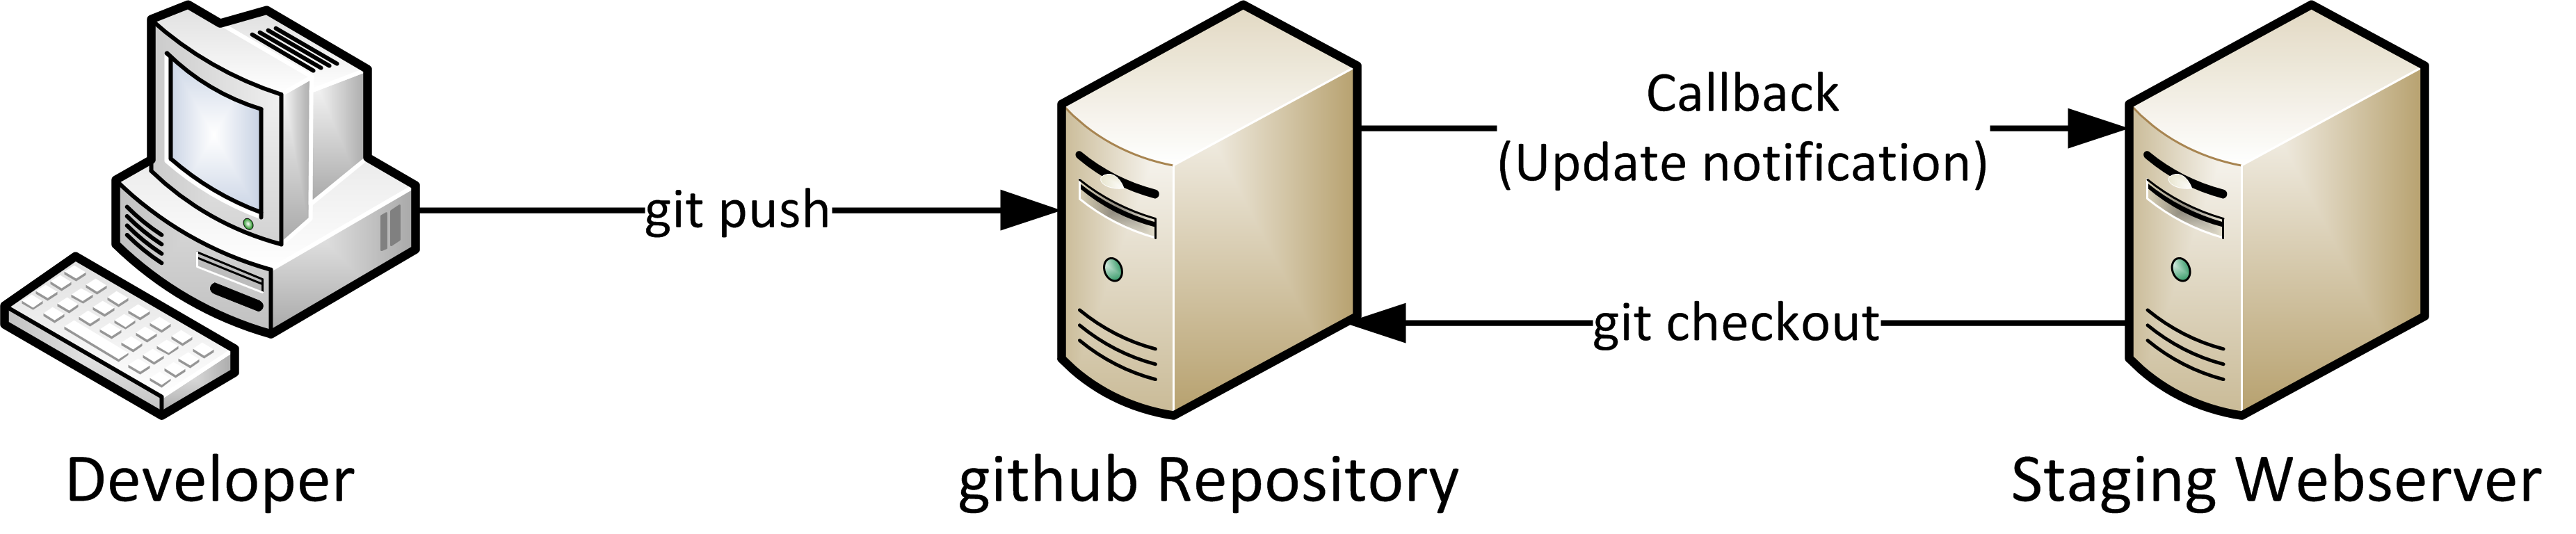
\includegraphics[width=\textwidth]{diagrams/staging-workflow.png}
  }
  \caption{Erster Entwurf des Forums}
  \label{}
\end{figure}

\lstset{language=bash}
\begin{lstlisting}[caption=Deployment script]
#!/bin/bash

cd /var/git/unplagged.git/
GIT_WORK_TREE=/var/www/preview.unplagged.com git checkout -f

cd /var/www/preview.unplagged.com
#generate phpdoc
apigen -s application/ -s library/Unplagged/ -d docs/phpdoc --title "Unplagged Documentation" --todo yes

#run database build scripts
cd scripts/build
php initdirectories.php
php doctrine_staging.php

cd /var/www
chown www-data:www-data preview.unplagged.com
\end{lstlisting}



\section{Architectural Goals}

\subsection{Progressive Enhancement}

\subsection{Test Driven Development}

\subsection{Responsive Design}